\section*{Das Perzeptron}

Der Aufbau eines typischen Perzeptrons besteht aus einer oder mehreren Schichten sogenannter \textit{Linear Threshold Units} (LTU) wie in Abbildung \ref{ltu} dargestellt.

\begin{figure}[ht]
	\begin{center}
		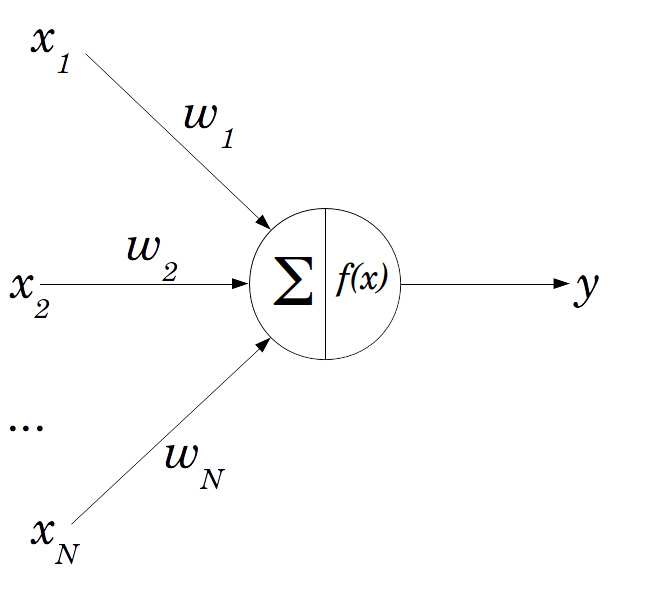
\includegraphics[width=9cm]{Bilder/perceptron.png} 
		\caption[Linear Threshold Unit]{Linear Threshold Unit \cite{AurelienGeron.2018}}
		\label{ltu}
	\end{center}
\end{figure}

Es besteht aus $n$ Eingängen mit $x_{i} \in \mathbb{Q}$, die im Inputvektor $\boldsymbol{x}$ zusammengefasst werden. Jeder Eingang wird mit einem Gewicht $w_{i}$ aus dem Gewichtsvektor $\boldsymbol{w}$ versehen \cite{AurelienGeron.2018}. Die LTU berechnet das Skalarprodukt $\boldsymbol{w}^{T} \circ \boldsymbol{x}$ aller Eingänge $\boldsymbol{x}$ mit ihren Gewichten $\boldsymbol{w}$ und wendet anschließend auf das Ergebnis $z$ eine Aktivierungsfunktion an \cite{AurelienGeron.2018}. Das Ergebnis $h_{w}(x)$ kann anschließend als Eingabe für ein weiteres Perzeptron dienen. Die einfachste Aktivierungsfunkion für ANNs ist die \textit{Heaviside-Funktion} \cite{AurelienGeron.2018}: 

\begin{equation} \label{heaviside}
\begin{split}
h_{w}(x) = s(\boldsymbol{w}^{T} \circ \boldsymbol{x}) = s(z) = \\\ \begin{pmatrix} 
w_{1}&&w_{2}&&\dots&& w_{n}\\ 
\end{pmatrix} 
\circ 
\begin{pmatrix} x_{1}\\
x_{2}\\
\vdots\\
x_{n}\\
\end{pmatrix}) = 
\begin{cases}
1 & \text{wenn} z \geq 0 \\
0 & \text{wenn} z < 0 .\\
\end{cases}
\end{split}
\end{equation}
\equations{Die Heaviside-Funktion}

Falls eine Klassifizierung mit Wahrscheinlichkeiten vorliegen soll, so ist die letzte Schicht eines Perzeptrons meist mit der \textit{Softmax-Funktion}

\begin{equation} \label{softmax}
h_{w}(x) = \sigma(z)_j = \frac{e^{z_j}}{\sum_{i=0}^n e^{z_i} }
\end{equation}
\equations{Die Softmax-Funktion}

implementiert, die den Wert des $j$-ten LTUs einer Schicht mit allen anderen $n$ Werten der LTUs derselben Schicht ins Verhältnis setzt \cite{AurelienGeron.2018}. Es gibt eine Vielzahl an möglichen Aktivierungsfunktionen, die im darauffolgenden Unterkapitel \textit{Hyperparameter} betrachtet werden.


Die Aktivierung einer LTU hängt zusätzlich von einem Schwellwert $\theta$ ab, der durch einen sogenannten \textit{Bias} festgelegt wird. Dies ist die Gewichtung des letzten Eingangs, der standardmäßig den Wert 1 liefert. Wird die Gewichtung negativ gewählt, so ist es schwieriger die LTU zu aktivieren, während eine positive Gewichtung die Aktivierung vereinfacht \cite{AurelienGeron.2018}.

Nun bilden ein oder mehrere Schichten solcher LTUs ein Perzeptron. Jede einzelne LTU ist dabei mit allen LTUs der vorherigen Schicht verbunden (siehe Abbildung \ref{neural_network}) \cite{AurelienGeron.2018}. Hier wird auch von sogenannten vollständig verbundenen Schichten (engl.: \textit{Fully-Connected Layer}) gesprochen. Die beiden LTUs zur Ausgabe können dabei Aussagen über eine Klassifikation von Daten anhand der Eingangsdaten treffen, während die LTUs im Input Layer wesentlich Daten weiter reichen. Die Verbindungen zur ersten Schicht des Hidden Layer sind stets mit Eins belegt. Existiert keine verborgene Schicht, so wird das \textit{Artificial Neural Network} (ANN) als einschichtiges Perzeptron bezeichnet, ab einer oder mehr verborgenen Schichten wird bereits von einem \textit{Multi-Layer Perzeptron} (MLP), einem mehrschichtigen Perzeptron, gesprochen \cite{AurelienGeron.2018}. Ist das neuronale Netz optimal trainiert, so ist am Ende nur eines der LTUs zur Ausgabe aktiviert. Das folgende ANN ist zudem ein Beispiel für ein sogenanntes \textit{Feed Forward Network}, bei dem die Auswertung der Daten von einer Schicht zur nächsten weitergereicht wird, ohne zu bereits besuchten Schichte zurückzukehren \cite{AurelienGeron.2018}.

\begin{figure}[ht]
	\begin{center}
		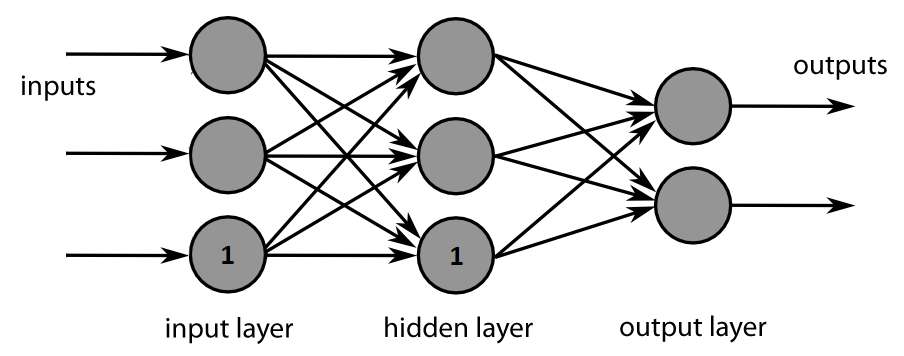
\includegraphics[width=12cm]{Bilder/neural_network.png} 
		\caption[Das einschichtige Perzeptron]{Das einschichtige Perzeptron \cite{Wikipedia.20190123}}
		\label{neural_network}
	\end{center}
\end{figure}